\chapter{Physical Activity and Health}\label{ch:g10:sport-and-health}

Two students are sixteen. One walks to school, plays basketball twice a
week and sleeps eight hours; the other is driven, spends the evening
seated in front of a screen, and sleeps six. At sixteen they look
similar. At fifty their doctors will see two different people: the
first with the heart, bones, muscles and blood sugar of someone twenty
years younger, the second with a list of conditions that begins with
the word "chronic". The three previous chapters have shown what a
working body does; this one is about what regular work does to it ---
and what abuse, in the form of overtraining or drugs, undoes.

\section{What training changes}

\begin{definition}[Physical activity and training]\label{def:g10:sport-and-health:training}
\emph{Physical activity}\index{physical activity} is any movement of
the body produced by the muscles that raises \omterm{def:g10:exercise-and-energy:expenditure}{energy expenditure} above
rest: walking, climbing stairs, housework, sport. \emph{Training} is
physical activity repeated with the aim of improving a capacity. The
body responds to a repeated demand by \emph{adapting}: enlarging,
strengthening or re-equipping the structures the demand loads ---
provided the demand is followed by the rest in which the adaptation
is built.
\end{definition}

\begin{proposition}[Adaptations to endurance training]\label{prop:g10:sport-and-health:endurance}
Repeated exercise of long duration and moderate intensity, over
months, produces:
\begin{itemize}
  \item a larger, stronger heart: the stroke volume rises, the resting
        rate falls (from 70 to 50 or below), the maximal output and the
        $\dot V\!\mathrm{O_2}$max increase by 10\% to 30\%;
  \item more capillaries and more \omterm{def:g10:cells-common-unit:organelle}{mitochondria} in the \omterm{def:g10:muscles-and-joints:muscle}{muscle fibres},
        which burn a larger share of fat and produce less lactic acid
        at a given power;
  \item more red blood \omterm{def:g10:cells-common-unit:cell}{cells}, hence more oxygen carried per litre;
  \item larger \omterm{def:g10:exercise-and-energy:glycogen}{glycogen} stores, and a body that regulates its blood
        sugar and its blood pressure more easily.
\end{itemize}
\end{proposition}
\admitted

\begin{omfigure}
\begin{tikzpicture}
\begin{axis}[
  width=0.86\linewidth, height=5.6cm,
  axis x line=bottom, axis y line=left,
  xmin=0, xmax=26, ymin=40, ymax=80,
  xlabel={weeks of training}, ylabel={resting heart rate (per min)},
  xlabel style={font=\small, at={(axis description cs:0.5,-0.12)}, anchor=north},
  ylabel style={font=\small},
  tick label style={font=\small}, xtick={0,4,8,12,16,20,24}, ytick={40,50,60,70,80},
  legend style={at={(0.5,-0.3)}, anchor=north, legend columns=2, font=\small, draw=none},
]
\addplot[thick, omThm, mark=*, mark size=1.5pt] coordinates
  {(0,72) (4,68) (8,64) (12,60) (16,57) (20,55) (24,54)};
\addplot[thick, omDef, mark=square*, mark size=1.5pt] coordinates
  {(0,72) (4,70) (8,66) (12,64) (16,62) (20,61) (24,61)};
\legend{4 sessions per week, 2 sessions per week}
\end{axis}
\end{tikzpicture}

{\small Resting heart rate of two groups of beginners over six months
of running. The fall reflects a growing stroke volume: the same
\qty{5}{L/min} at rest in fewer beats. Adaptation is proportional to
the demand, and slows as the body approaches its new state.}
\end{omfigure}

\begin{example}[The numbers of adaptation]\label{ex:g10:sport-and-health:numbers}
A sedentary 17-year-old with a $\dot V\!\mathrm{O_2}$max of
\qty{40}{mL/min} per kilogram runs three times a week for six months:
\num{48}, and a resting heart rate down from 72 to 58. His muscle
biopsy shows 40\% more \omterm{def:g10:cells-common-unit:organelle}{mitochondria} and 30\% more capillaries per
fibre. His fibres are the same in number and the same in type; they
have been re-equipped.
\end{example}

\begin{proposition}[Adaptations to strength training]\label{prop:g10:sport-and-health:strength}
Repeated contractions against heavy loads thicken the \omterm{def:g10:muscles-and-joints:muscle}{muscle fibres}
(more myofibrils in each) and improve the nervous command that
recruits them; strength can double in a year while the number of
fibres does not change. The \omterm{def:g10:muscles-and-joints:muscle}{tendons} and the bones loaded by the
training thicken too, more slowly. Bone, in particular, is built and
maintained in response to the loads it carries: an active adolescence
sets the bone mass that will be drawn down in old age, and a limb
immobilised in a cast loses bone within weeks.
\end{proposition}
\admitted

\section{Activity and health}

\begin{proposition}[Effects of regular activity on health]\label{prop:g10:sport-and-health:health}
Regular \omterm{def:g10:sport-and-health:training}{physical activity} --- the equivalent of an hour a day of
moderate activity for adolescents, half an hour for adults --- lowers
the risk of the commonest chronic diseases: heart and artery disease,
type 2 diabetes, several cancers, osteoporosis, depression. It does so
through the adaptations above: a heart and vessels that work at lower
pressure, muscles that draw glucose from the blood readily, bones that
keep their mass, a body mass kept within a healthy range. The effect
is large --- comparable to that of not smoking --- and it does not
require sport, only movement.
\end{proposition}
\begin{proof}[Evidence]
Studies following tens of thousands of people for decades find that
those in the most active fifth of the population die, at a given age,
at about half the rate of those in the least active fifth, with heart
disease accounting for most of the difference; the relation holds
after allowing for diet, smoking and social conditions, and it is
graded --- each step up in activity brings a step down in risk. Trials
in which sedentary people are assigned to a walking programme show
falls in blood pressure and blood sugar within months.
\end{proof}

\begin{omfigure}
\begin{tikzpicture}
\begin{axis}[
  ybar, bar width=16pt,
  width=0.8\linewidth, height=5.4cm,
  axis x line=bottom, axis y line=left,
  ymin=0, ymax=1.2, ylabel={relative risk of death},
  ylabel style={font=\small},
  symbolic x coords={least active, low, moderate, high, most active},
  xtick=data, tick label style={font=\small},
  xlabel={fifths of the population by weekly activity},
  xlabel style={font=\small, at={(axis description cs:0.5,-0.14)}, anchor=north},
  enlarge x limits=0.15, ytick={0,0.2,0.4,0.6,0.8,1.0},
  nodes near coords, nodes near coords style={font=\scriptsize},
  every node near coord/.append style={/pgf/number format/fixed, /pgf/number format/precision=2},
]
\addplot[fill=omThm!50, draw=omThm] coordinates
  {(least active,1.00) (low,0.80) (moderate,0.70) (high,0.62) (most active,0.55)};
\end{axis}
\end{tikzpicture}

{\small Risk of death over a follow-up of twenty years, relative to the
least active fifth, in a large adult population (rounded from several
studies). Each step of activity lowers the risk; the largest gain is
the first, from none to some.}
\end{omfigure}

\begin{example}[Blood sugar and muscle]\label{ex:g10:sport-and-health:sugar}
A muscle at work takes glucose from the blood without needing the
hormone insulin, and a trained muscle stays more sensitive to insulin
between sessions. A brisk walk after a meal lowers the peak of blood
glucose that follows it; a sedentary body, asked to store the same
sugar without moving, needs more insulin each year --- the road to type
2 diabetes, whose mechanism is the subject of the final year.
\end{example}

\section{Too much, too fast, too wrong}

\begin{proposition}[Overtraining and injury]\label{prop:g10:sport-and-health:overtraining}
Adaptation is built during rest. A demand repeated without enough
recovery --- more sessions, or heavier ones, than the tissues can
repair between them --- produces the reverse of adaptation:
persistent fatigue, a rising resting heart rate, falling performance,
disturbed sleep, frequent infections, and, in the tissues that repair
slowest (\cref{ch:g10:muscles-and-joints}), tendinitis and stress
fractures. The commonest cause of injury in adolescents is not the
sport but the rate at which its load is increased.
\end{proposition}
\admitted

\begin{example}[The rule of ten per cent]\label{ex:g10:sport-and-health:tenpercent}
A runner who increases her weekly distance by no more than 10\% a
week rarely hurts herself; one who doubles it in a fortnight often
does. Bone and \omterm{def:g10:muscles-and-joints:muscle}{tendon} adapt over months, muscle and heart over
weeks: the slow tissues set the pace at which the load may rise.
\end{example}

\begin{proposition}[Doping]\label{prop:g10:sport-and-health:doping}
\emph{Doping}\index{doping} is the use of substances or methods that
raise performance by acting on the body's regulation, in place of the
adaptation training would build. Each one imitates an adaptation and
carries the cost of bypassing it:
\begin{itemize}
  \item the hormone erythropoietin (EPO), or transfusion of one's own
        stored blood, raises the number of red blood \omterm{def:g10:cells-common-unit:cell}{cells} --- and
        thickens the blood until it can clot in the vessels of the
        heart or brain;
  \item anabolic steroids, derived from testosterone, thicken \omterm{def:g10:muscles-and-joints:muscle}{muscle
        fibres} --- and disturb the body's own hormones, the liver, the
        heart and the mood;
  \item stimulants mask fatigue --- and remove the warning that
        protects the heart from overheating and exhaustion;
  \item growth hormone, and drugs that hide the others, complete the
        list.
\end{itemize}
\omterm{prop:g10:sport-and-health:doping}{Doping} is forbidden in competition because it is unfair; it is
dangerous because every one of these substances overrides a
regulation that exists for a reason.
\end{proposition}
\admitted

\begin{example}[EPO in numbers]\label{ex:g10:sport-and-health:epo}
Red blood \omterm{def:g10:cells-common-unit:cell}{cells} make about 45\% of the volume of normal blood. EPO
abuse has pushed athletes to 55\% and beyond, a blood so thick that
the heart, slowed by sleep, cannot move it: several young cyclists
died in their sleep in the years before tests existed. \omterm{def:g10:sport-and-health:training}{Training} at
altitude raises the same figure by two or three points, over weeks,
under the body's own control.
\end{example}

\section{The everyday rules}

\begin{method}[Training safely]\label{met:g10:sport-and-health:rules}
\begin{enumerate}
  \item \emph{Progress slowly}: increase the load by about a tenth a
        week, and let bone and \omterm{def:g10:muscles-and-joints:muscle}{tendon} set the pace.
  \item \emph{Warm up and cool down}: ten minutes each, for the reasons
        of \cref{ch:g10:muscles-and-joints}.
  \item \emph{Drink}: an hour of hard exercise loses one to two litres
        of sweat; replace it, with some salt, before thirst says so ---
        a loss of 2\% of body mass already lowers performance.
  \item \emph{Eat for the effort}: \omterm{def:g10:chemistry-of-life:families}{carbohydrates} before and during long
        efforts, \omterm{def:g10:chemistry-of-life:families}{proteins} for repair afterwards
        (\cref{ch:g10:exercise-and-energy}); no supplement replaces a
        varied diet.
  \item \emph{Rest}: sleep is when adaptation is built; a rising
        resting heart rate is the earliest sign of too little.
  \item \emph{Listen to pain}: sharp pain in a \omterm{def:g10:muscles-and-joints:joint}{joint} or \omterm{def:g10:muscles-and-joints:muscle}{tendon} is a
        signal, not an obstacle.
\end{enumerate}
\end{method}

\begin{omfigure}
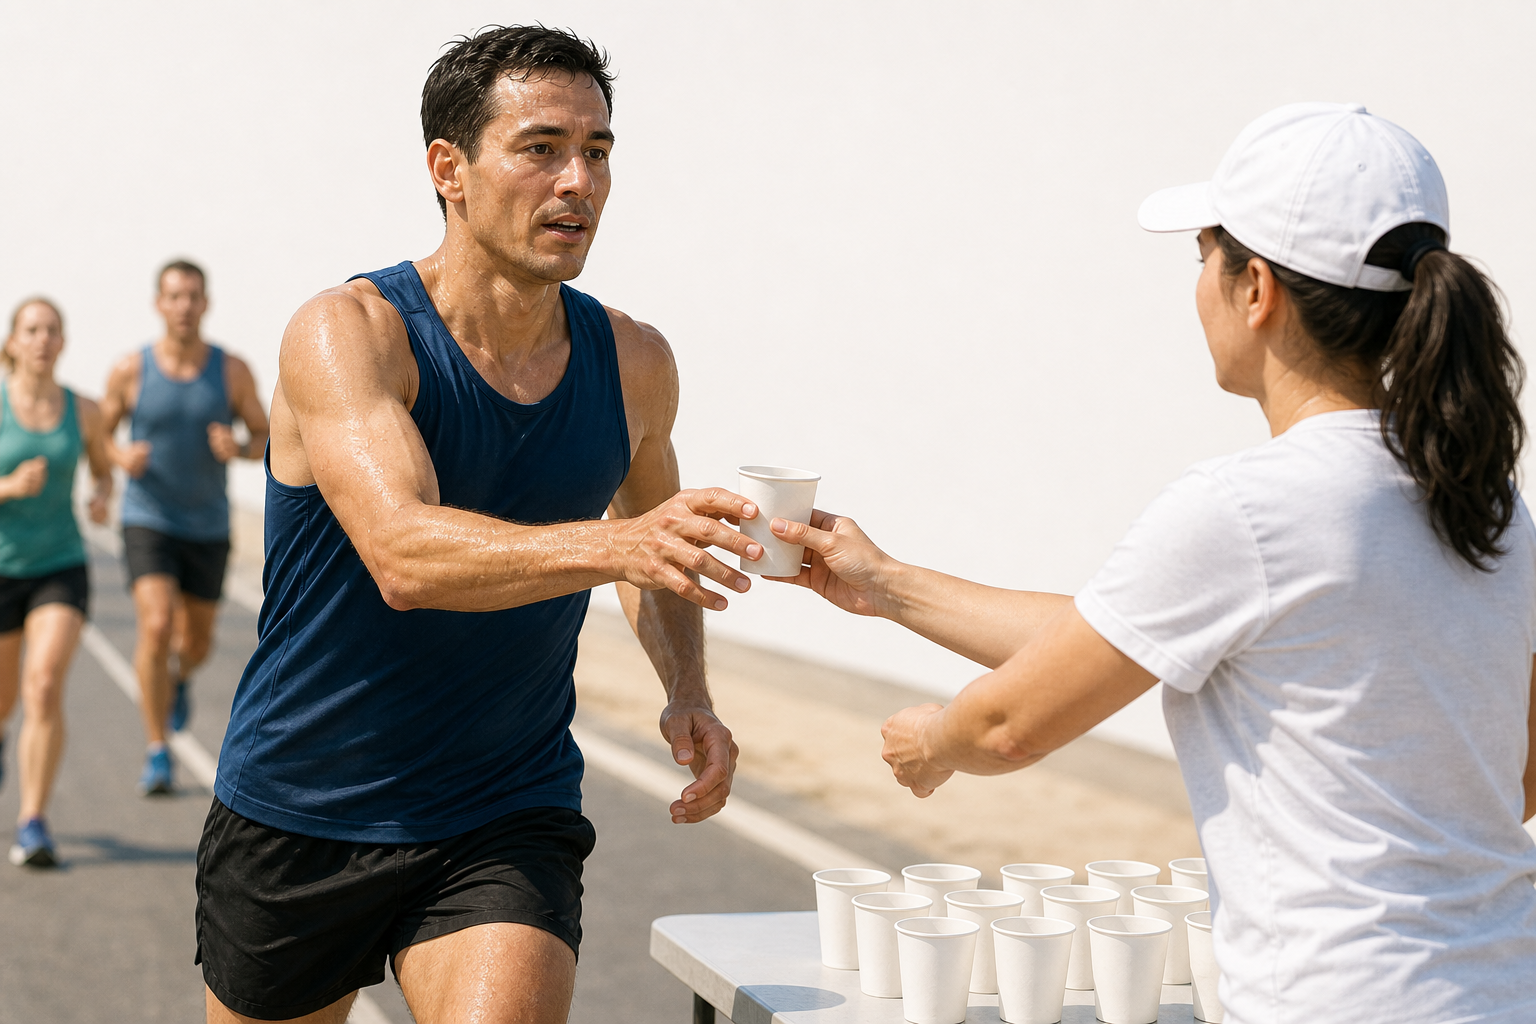
\includegraphics[width=0.62\linewidth]{images/book2/ai/g10-health-hydration.png}

{\small An aid station on a marathon course. At a sweating rate of
over a litre an hour, the water lost must be replaced during the
effort; waiting for thirst means running already dehydrated.}
\end{omfigure}

\begin{example}[Hydration in numbers]\label{ex:g10:sport-and-health:water}
A \qty{60}{kg} runner sweats \qty{1.2}{L} per hour in warm weather. In
a two-hour run she loses \qty{2.4}{kg}, 4\% of her mass: her blood
volume falls, her heart rate rises by ten beats to keep the output,
her body temperature climbs, and her pace drops by a tenth. Drinking
half a litre an hour would have halved the loss.
\end{example}

\begin{remark}[The body keeps the account]\label{rem:g10:sport-and-health:account}
Every adaptation of this chapter is a structure the body builds in
response to use, and every one of them is dismantled again when the
use stops: a month in bed loses a fifth of the muscle, a year of
inactivity loses most of the endurance gains. The account is kept
continuously, and the balance at fifty is the sum of the deposits
made at sixteen, twenty-six and thirty-six.
\end{remark}

\section{Exercises}

\begin{exercise}[$\star$]\label{exo:g10:sport-and-health:1}
List four adaptations of the body to endurance training.
\end{exercise}

\begin{exercise}[$\star$]\label{exo:g10:sport-and-health:2}
Why does the resting heart rate fall with training, although the
resting \omterm{def:g10:heart-lungs-effort:output}{cardiac output} does not change?
\end{exercise}

\begin{exercise}[$\star$]\label{exo:g10:sport-and-health:3}
What is the recommended daily amount of \omterm{def:g10:sport-and-health:training}{physical activity} for an
adolescent? Does it have to be sport?
\end{exercise}

\begin{exercise}[$\star$]\label{exo:g10:sport-and-health:4}
Define doping and give two examples with the regulation each one
overrides.
\end{exercise}

\begin{exercise}[$\star$]\label{exo:g10:sport-and-health:5}
Name three signs of overtraining.
\end{exercise}

\begin{exercise}[$\star\star$]\label{exo:g10:sport-and-health:6}
From the heart-rate figure, compare the fall after 12 weeks in the two
groups, and say what it shows about the relation between demand and
adaptation.
\end{exercise}

\begin{exercise}[$\star\star$]\label{exo:g10:sport-and-health:7}
A runner's resting output is \qty{5.0}{L/min}. Her resting heart rate
falls from 72 to 54 over six months. By what factor did her stroke
volume change?
\end{exercise}

\begin{exercise}[$\star\star$]\label{exo:g10:sport-and-health:8}
From the relative-risk figure, by what fraction is the risk of death
lower in the most active fifth than in the least active? Which single
step brings the largest gain?
\end{exercise}

\begin{exercise}[$\star\star$]\label{exo:g10:sport-and-health:9}
A \qty{55}{kg} student plays a two-hour tennis match in summer,
sweating \qty{1.0}{L} per hour and drinking nothing. What fraction of
her mass has she lost, and what are three consequences?
\end{exercise}

\begin{exercise}[$\star\star$]\label{exo:g10:sport-and-health:10}
A beginner runs \qty{10}{km} a week. Following the rule of ten per
cent, how many weeks does it take to reach \qty{20}{km} a week?
(Compute week by week, or note that $1.1^7 \approx 1.95$.)
\end{exercise}

\begin{exercise}[$\star\star$]\label{exo:g10:sport-and-health:11}
Explain why muscle strength can double in a year of training while
the number of \omterm{def:g10:muscles-and-joints:muscle}{muscle fibres} stays the same.
\end{exercise}

\begin{exercise}[$\star\star\star$]\label{exo:g10:sport-and-health:12}
An athlete's blood has 45\% red \omterm{def:g10:cells-common-unit:cell}{cells}; after EPO abuse, 56\%. Using
\cref{ch:g10:heart-lungs-effort}, estimate the gain in oxygen carried
per litre and hence in $\dot V\!\mathrm{O_2}$max, and explain why the
gain is bought at the risk of a fatal clot.
\end{exercise}

\begin{exercise}[$\star\star\star$]\label{exo:g10:sport-and-health:13}
\omterm{def:g10:sport-and-health:training}{Training} at altitude for three weeks raises red \omterm{def:g10:cells-common-unit:cell}{cells} from 45\% to
48\%; EPO raises them to 56\% in the same time. In what sense is the
first an adaptation and the second not, although the molecule involved
is the same?
\end{exercise}

\begin{exercise}[$\star\star\star$]\label{exo:g10:sport-and-health:14}
Explain, using \cref{ex:g10:sport-and-health:sugar}, why doctors
prescribe walking to patients whose blood sugar is beginning to rise,
and why the prescription works better than a drug that only lowers the
sugar.
\end{exercise}

\begin{exercise}[$\star\star\star$]\label{exo:g10:sport-and-health:15}
"A month of intensive training before the exam season will set me up
for the year." Discuss with the notions of adaptation, rest, and the
time scales of the different tissues.
\end{exercise}

\section{Problem: Two Students, Thirty Years}

\begin{problem}[{Weekend problem --- an active and a sedentary
sixteen-year-old followed through training, a season of overtraining,
and the accounts their bodies keep to middle age}]
\label{pb:g10:sport-and-health:1}
Alex and Sam are sixteen, both \qty{62}{kg}, both with a resting heart
rate of 72 and a $\dot V\!\mathrm{O_2}$max of \qty{42}{mL/min} per
kilogram. Alex starts running three times a week; Sam does not.

\medskip
\noindent\textbf{Part I --- Alex trains.}
After six months Alex's resting heart rate is 56 and his
$\dot V\!\mathrm{O_2}$max \qty{50}{mL/min} per kilogram; his maximal
heart rate (200) has not changed.
\begin{enumerate}
  \item His resting \omterm{def:g10:heart-lungs-effort:output}{cardiac output} is still \qty{4.8}{L/min}. Compute
        his stroke volume before and after.
  \item Compute his $\dot V\!\mathrm{O_2}$max in litres per minute
        before and after, and the percentage gain.
  \item Assuming his maximal oxygen extraction (\qty{150}{mL} per
        litre) has not changed, compute his maximal \omterm{def:g10:heart-lungs-effort:output}{cardiac output}
        before and after, and his maximal stroke volume before and
        after.
  \item Which of the adaptations of
        \cref{prop:g10:sport-and-health:endurance} explains the gain in
        stroke volume, and which one would explain a gain in
        extraction?
  \item Alex's weekly distance went from \qty{6}{km} to \qty{24}{km}
        in six months. Was the rule of ten per cent respected? Show
        the calculation.
\end{enumerate}

\medskip
\noindent\textbf{Part II --- Alex overtrains.}
In the spring Alex doubles his distance in two weeks to prepare a
race. Three weeks later: resting heart rate 64, poor sleep, a cold, a
pain in the shin, slower race times.
\begin{enumerate}[resume]
  \item Name the condition and list the signs from the chapter that
        match.
  \item What is the most likely cause of the shin pain, in the
        vocabulary of \cref{ch:g10:muscles-and-joints}, and why that
        tissue?
  \item Why does the resting heart rate rise, when training had
        lowered it?
  \item Propose a three-week plan and justify each element with
        \cref{met:g10:sport-and-health:rules}.
  \item A teammate offers a "supplement" that removes tiredness. Which
        category of \cref{prop:g10:sport-and-health:doping} does it
        belong to, and what regulation does it override?
\end{enumerate}

\medskip
\noindent\textbf{Part III --- Sam sits.}
At thirty Sam is \qty{80}{kg}, with a resting heart rate of 78 and a
$\dot V\!\mathrm{O_2}$max of \qty{32}{mL/min} per kilogram; Alex, still
active, is \qty{64}{kg}, 54 and \num{48}.
\begin{enumerate}[resume]
  \item Compute both men's $\dot V\!\mathrm{O_2}$max in litres per
        minute. Which absolute value is larger, and why is the
        per-kilogram figure the one that matters for daily life?
  \item Climbing four flights of stairs costs each man about
        \qty{12}{mL} of oxygen per kilogram per minute above rest.
        What fraction of his maximum does each use? Who arrives out of
        breath?
  \item Sam's doctor finds a blood sugar slightly above normal.
        Explain, with \cref{ex:g10:sport-and-health:sugar}, the link
        with his inactivity.
  \item The doctor prescribes half an hour of brisk walking a day.
        Using the relative-risk figure, estimate the reduction in
        long-term risk if Sam moves from the least active fifth to the
        moderate one.
  \item Sam objects that he has no time for sport. Answer him with
        \cref{def:g10:sport-and-health:training}.
\end{enumerate}

\medskip
\noindent\textbf{Part IV --- The account at fifty.}
\begin{enumerate}[resume]
  \item Bone mass peaks around twenty-five and then declines by about
        1\% a year. If Alex's peak was 10\% higher than Sam's because
        of his active adolescence, how many years of decline does that
        margin represent?
  \item After a fall at fifty, Sam fractures a wrist and Alex does
        not. Relate this to question 16 and to
        \cref{prop:g10:sport-and-health:strength}.
  \item Alex broke his training for a year at forty after an injury
        and lost most of his endurance gains, then rebuilt them. What
        does this show about the nature of an adaptation?
  \item List, for Sam at fifty, three conditions of
        \cref{prop:g10:sport-and-health:health} his inactivity has made
        more likely, and the mechanism of one of them.
  \item State the result: the two numbers (resting heart rate,
        $\dot V\!\mathrm{O_2}$max per kilogram) that separate the two
        men at thirty, and the one habit, stated in hours per week,
        that produced the difference.
\end{enumerate}
\end{problem}
